
%OFDM PAPR 


\documentclass[20pt,landscape]{foils}
\usepackage[pdftex]{color}
\usepackage[pdftex]{graphicx}
\usepackage[pdftex]{geometry}
\geometry{headsep=2ex,hscale=0.9} \pdfpagewidth=11in
\pdfpageheight=8.5in

\setlength{\footskip}{0.0in} \setlength{\textheight}{8.0in}

\usepackage{background}
\usepackage{pp4slide}
%\usepackage{pdfscreen}

\newcommand{\bx}{{\mbox {\boldmath $x$}}}
\newcommand{\bv}{{\mbox {\boldmath $v$}}}
\newcommand{\ba}{{\mbox {\boldmath $a$}}}
\newcommand{\bb}{{\mbox {\boldmath $b$}}}
\newcommand{\bA}{{\mbox {\boldmath $A$}}}
\newcommand{\bH}{{\mbox {\boldmath $H$}}}
\newcommand{\bG}{{\mbox {\boldmath $G$}}}
\newcommand{\bM}{{\mbox {\boldmath $M$}}}
\newcommand{\bN}{{\mbox {\boldmath $N$}}}
\newcommand{\balpha}{{\mbox {\boldmath $\alpha$}}}
\newcommand{\bbeta}{{\mbox {\boldmath $\beta$}}}
\newcommand{\bgamma}{{\mbox {\boldmath $\gamma$}}}



\zerolistvertdimens

\begin{document}
%\raggedright \color{white}, change back when finnalizing.
\raggedright \color{black}
\definecolor{bgcolor}{rgb}{0.04,0.37,0.59}
\pagecolor{bgcolor} % set background color
\definecolor{bgblue}{rgb}{0.04,0.37,0.59}
\vpagecolor{bgblue}


\foilhead{\LARGE A New Distribution Bound and  \\
Reduction Scheme for OFDM PAPR}

\begin{center}
\vspace{.3in}

{\bf X. Zhou \& Dr. J. Caffery, Jr.}  \\
{\it University of Cincinnati \\ Dept. of Electrical \& Computer
Engineering \\ \& Computer Science \\ Cincinnati,
OH~~45221-0030} \\
\vspace{.5in}
\end{center}

%First slide, general intro and motivations
\foilhead[-0.5in]{Introduction}
\begin{itemize}
\item The demand of high data rate over the wireless
channel.\vspace{-0.25in}
    \begin{itemize}
    \item Wireless multimedia $>$2 Mbps
    \item 2-155 Mbps under investigation
    \end{itemize} \vspace{-0.25in}

\item Some applications:\vspace{-0.25in}
\begin{itemize}
    \item DAB (useful bit rate 5.6 Mbps)
    \item DVB over the terrestrial networks, digital terrestrial television broadcasting
(DTTB)
 \item HIPERLAN Phase II, supporting 20 Mbps in propagation environments
with delay spreads up to 1 us
 \item IEEE 802.11A (48 subcarriers, 5,10,15,20,30 Mbps.)
\item Asymmetric digital subscriber Line (ADSL) \item High speed
cellular (Band Division Multiple Access, BDMA)
\end{itemize} \vspace{-0.25in}

\item How to transmit a large bit stream over a wireless channel
to provide sufficient QoS? What modulation can be
used?\vspace{-0.30in}

\item Wireless environment channel is harsh (path loss, shadowing,
multipath, etc.).\vspace{-0.30in}

\item Possible solutions to high bit rate transmission over
wireless channels?\vspace{-0.30in}
\end{itemize}


%second slide, talk about the possible solution for high data rate
\foilhead[-0.5in]{Possible Solutions for High Data Rate
Transmission}
\begin{itemize}
\item Possible Solutions are \vspace{-.2in}

 \begin{itemize}

 \item {\bf Equalization} --- Practical difficulties in performing equalization in real-time at several Mbps with
low complexity and compact hardware.

 \item {\bf Spread spectrum} --- Robust against fading, interference. However, if data rate is 20 Mbps, the
spreading factor is 128, then 2.56Gcps; another difficulty is
near-far problem.

 \item {\bf Ultra wide band (UWB)} --- High capacity, multipath-fading resistant, immunity to impulse noise,
hard to design the hardware to accommodate the very wide frequency
range, hard to design antenna, interference with existing GPS, RF
devices? FCC approval.

\item {\bf Multicarrier/OFDM} --- The transmission bandwidth $B$
with data rate $R$ is divided into many ($N$) narrow subchannels.
Each subchannel has bandwidth $B/N$ and date rate $R/N$. All
subchannels contribute the high bit rate in parallel. For the
end-users, a high bit rate is achieved!.

 \vspace{-.25in}
 \end{itemize}
\item As a special and important form of multicarrier, OFDM is
implemented via IFFT/FFT in MODEM.
\end{itemize}


%the third slide, in this slide, highlight the features of OFDM and give the math model
\foilhead[-0.5in]{OFDM System Model}

\begin{itemize}
\item Use IFFT/FFT to modulate/demodulate,reduces the complexity
of MC. \vspace{-.25in}

\item Carrier spacing is the reciprocal of the useful OFDM symbol
period $T$. \vspace{-.25in}

\item OFDM is a particular form of MC with overlapping orthogonal
subcarriers.\vspace{-.25in}

\item The continuous time OFDM signal, in one symbol period, is
given by\vspace{-.25in}
$$
s\left( t \right) = \frac{1}{{\sqrt N }}\sum\limits_{k = 0}^{N -
1} {S_k e^{j2\pi kt/T} g(t)}
$$
where $S_k $ is the QAM value of the $k^{th}$ subcarrier, $g(t)$
is the rectangular window of unit height over the OFDM symbol
interval $[0,T]$ and $N$ is the subcarrier number.\vspace{-.25in}

\item The Nyquist-rate sampled OFDM signal is given
by\vspace{-.25in}
$$
s_n  = \frac{1}{{\sqrt N }}\sum\limits_{k = 0}^{N - 1} {S_k
e^{j2\pi kn/N} }.
$$
\end{itemize}


%This is the fourth slide, here give the PAPR problem formulation
\foilhead[-0.5in]{PAPR Problem Formulation}
\begin{itemize}
\item An OFDM signal is the sum of independently modulated
subcarrier signals.\vspace{-.25in}

 \item If those subcarriers are added coherently, the total
instantaneous power will become much larger than the average
power.\vspace{-.25in}

\item Therefore, RF power amplifiers should operate in a very
large linear region. Otherwise, if signal peaks move into the
nonlinear region of the power amplifier, signal distortion results
by introducing intermodulation among the subcarriers and
out-of-band radiation. Thus, it is highly desirable to reduce the
PAPR.\vspace{-.25in}

\item The PAPR of the OFDM signal $s_\tau$, where $\tau$ is used
to represent both the continuous time index $t$ and discrete time
index $n$, is defined as\vspace{-.35in}
$$
{\rm PAPR\/}\{ s_\tau  ,\xi \}  = \frac{{\mathop {\max
}\limits_{\tau  \in \xi } \left| {s_\tau  } \right|^2 }}{{E\{
\left| {s_\tau  } \right|^2 \} }} \vspace{-.35in}$$ where $\xi$
denotes either $T$ or $N$.\vspace{-.35in}

\item PAPR distribution is better to describe the PAPR
characteristics than the maximum PAPR in practical OFDM systems.
\end{itemize}



%this is the 5th slide,  to present some assumptions.
\foilhead[-0.5in]{Assumptions and Observations}
\begin{itemize}
\item Guard time is an important issue in OFDM systems, however it
is just a partial replica of the signal during $[0,T]$, it changes
neither the average nor peak power of the signal. Thus, it is removed in our analysis.

\item Since the RF frequency is much higher than the subcarrier's
frequency,  the baseband OFDM signal has the same PAPR as its
passband equivalent, so we use the baseband signal to analyze the
PAPR.

\item We assume an ideal bandlimited OFDM signal where the
bandwidth $B = N/T$ and its power spectral density (PSD) is
constant over $\left[ { - B/2,B/2} \right]$.

\item The baseband OFDM signal, $s(t)$, can be written in complex
form as $s(t)=x(t)+jy(t)$. According to Central Limit Theorem,
$x(t)$ and $y(t)$ can be approximated as two independent Gaussian
random processes and the envelope of $s(t)$ can be approximated as
Rayleigh process.
\end{itemize}

%slide 6, give PAPR CCDF definition.
\foilhead[-0.5in]{PAPR Distribution}
\begin{itemize}
\item Define the normalized OFDM signal and PAPR cumulative CDF as
followings:\vspace{-.15in}
$$
r(t) = \frac{{s(t)}}{{\sqrt {P_{AV} } }} = \frac{{x(t) +
jy(t)}}{{\sqrt {P_{AV} } }}
$$
where $P_{AV}  = E[\left| {s(t)} \right|^2 ]$ denotes the average
power over the entire signal. Thus, $\left| {r(t)} \right|$ is
also approximated by a Raleigh process.\vspace{-.25in}

\item The PAPR cumulative CDF is defined as:\vspace{-.15in}
$$
C_{{\rm PAPR\/}} (\gamma ) = \Pr \left\{ \mathop {\max }\limits_{0
< t < T} \left| {r(t)} \right|^2  \ge \gamma \right\}
$$ where $T$ denotes one OFDM symbol period.\vspace{-.25in}

\item It is straightforward that\vspace{-.15in}
$$
C_{{\rm PAPR\/}} (\gamma ) = \Pr \left\{ \mathop {\max }\limits_{0
< t < T} \left| {r(t)} \right|^{}  \ge \sqrt \gamma \right\}.
$$
\end{itemize}


%slide 7, give previous results on PAPR distribution
\foilhead[-0.4in]{Previous Bounds or Approximations}
\begin{itemize}
\item  According to the Rayleigh distribution and Nyquist sampling
rate,  van Nee and de Wild (1998) gave a $lower
bound$ and an $experimental approximation$ as\vspace{-.45in}
$$
C_{{\rm PAPR\/}} (\gamma ) \ge 1-(1 - e^{ - \gamma }
)^N,$$ \vspace{-0.4in}  $$  C_{{\rm PAPR\/}} (\gamma ) = 1-(1 - e^{ - \gamma }
)^{2.8N}.
$$ \vspace{-0.5in}


\item An $upper bound$ based on oversampled signals is proposed
by Sharif and Khalaj (2001)  as\vspace{-.25in}
$$
C_{{\rm PAPR\/}} ({\rm PAPR\/} > \gamma ) \le k_{opt} Ne^{ -
\gamma (1 - {\raise0.7ex\hbox{$\pi $} \!\mathord{\left/
 {\vphantom {\pi  {k_{opt} }}}\right.\kern-\nulldelimiterspace}
\!\lower0.7ex\hbox{${k_{opt} }$}})}.
$$ \vspace{-0.35in}
where $k_{opt}  > \pi$ and $\frac{\pi }{{k_{opt} }}(1 - \frac{\pi
}{{k_{opt} }}) = \frac{1}{\gamma }.$\vspace{0.1in}


\item  Using the level crossing rate approach and numerical
computations, an $approximation$ of the PAPR CCDF is given by
Ochiai and Imai (2001) as:\vspace{-.20in}
$$
C_{{\rm PAPR\/}} (\gamma ) = \left\{ {\begin{array}{*{20}c}
   {1-(1 - \frac{{\sqrt \gamma  e^{ - \gamma } }}{{\sqrt {\overline \gamma  } e^{ - \overline \gamma  } }})^{\sqrt {\frac{\pi }{3}} N\sqrt {\overline \gamma  } e^{ - \overline \gamma  } } ,\begin{array}{*{20}c}
    & {\gamma  > \overline \gamma  }  \\
\end{array}}  \\
   {1,\begin{array}{*{20}c}
   {\begin{array}{*{20}c}
   {} & {}  \\
\end{array}\begin{array}{*{20}c}
   {\begin{array}{*{20}c}
   {\begin{array}{*{20}c}
   {} & {}  \\
\end{array}} & {}  \\
\end{array}} & {\begin{array}{*{20}c}
   {} & {}  \\
\end{array}}  \\
\end{array}} & {\gamma  \le \overline \gamma  }  \\
\end{array}}  \\
\end{array}} \right.
$$ where $\overline \gamma$ stands for the reference PAPR value whose
probability is negligible (close to 0).\vspace{-.4in}



\end{itemize}


%slide 8, new PAPR bound idea

\foilhead[-0.5in]{A New Simple Upper Bound}
\begin{itemize}

\item One peak occurs if there is a positive level crossing at the
same amplitude value. Thus,  the probability that the PAPR is
greater than $\gamma^2 $ is equivalent to the probability that
$\left| {r(t)} \right|$ will cross $\gamma$ at least once during one OFDM symbol
period $T$ $($The level crossing adopted is the one with positive
slope.$)$.\vspace{-.25in}

\item $ \Pr\left\{ \mathop {\max }\limits_{0 < t < T } \left|
{r(t)}^2 \right|
> \gamma^2 \right\}  = \Pr[C_{r } (\gamma ,T ) \ge 1]
$ ~where $C_{r  } (\gamma ,T )$ denotes the number of times that
$r(t)$ crosses level $\gamma$ during time period
$T$.\vspace{-.25in}

\item Use the Markov inequality to convert the above into an
inequality
$$
\Pr\left\{ \mathop {\max }\limits_{0 < t < T } \left| {r(t)}
\right|
> \gamma \right\}  \le E[C_{r } (\gamma ,T )].\vspace{-.15in}
$$Thus,  $E[C_{r} (\gamma ,T )]$, the mean number of
crossings at level $\gamma$, denotes an upper bound of the crest
factor CCDF.
\end{itemize}


%slide 9, derivation of the bound
\foilhead[-0.5in]{Derivation of the Upper Bound}
\begin{itemize}
\item The level crossing rate of a Rayleigh or Ricean process $v_r
(\gamma )$ is given  by:
$$
v_r (\gamma ) = \sqrt {\frac{{b_2 }}{{b_0 }} - \frac{{b_1 ^2
}}{{b_0^2 }}} \frac{{\gamma e^{ - \gamma ^2 } }}{{\sqrt \pi  }}
$$ where the $n^{th}$ spectral moment $b_n$ is defined as
$$
b_n  = \left. {\frac{{d^n \phi(\tau)}}{{j^n d\tau ^n }}}
\right|_{\tau = 0}
$$
and $\phi(\tau)$, the autocovariance of $r(t)$, is defined as
$$
\phi(\tau) = \frac{{E[r^* (t)r(t + \tau )] - \left| {E[r(t)]}
\right|^2 }}{2}.
$$
\end{itemize}

%slide 10, the final results
\foilhead[-0.5in]{Final Result}
\begin{itemize}
\item $x(t)$ and $y(t)$ are  uncorrelated and have the same
autocorrelation function as $R_x (\tau ) = R_y (\tau ).$
\vspace{-.25in}

\item For the Rayleigh process, we have $\phi(\tau ) = R_x (\tau
).$\vspace{-.25in}

\item  If  $S_x(f)$  denotes the PSD of $x(t)$, then  $ R_x (\tau
) = \int\limits_{ - \infty }^\infty {S_x (f)e^{j2\pi f\tau }
df}.$\vspace{-.25in}

\item Further, $b_n  = (2\pi )^n \int\limits_{ - \infty }^\infty
{S_x (f)f^n df}.$ \vspace{-.25in}

\item For an ideal bandlimited OFDM signal, the PSD of $x(t)$ is
expressed by\vspace{-.15in}
$$
S_x (f) = \left\{ {\begin{array}{*{20}c}
   H  \\
   0  \\
\end{array}} \right.\begin{array}{*{20}c}
   {}  \\
   {}  \\
\end{array}\begin{array}{*{20}c}
   {}  \\
   {}  \\
\end{array}\begin{array}{*{20}c}
   {\left| f \right| \le B/2}  \\
   {\left| f \right| > B/2}  \\
\end{array}
$$where $H$ is a constant and $B$ is the bandwidth.\vspace{-.25in}

\item The PAPR CCDF bound is obtained as \vspace{-.25in}
$$C_{{\rm PAPR\/}} (\gamma ) \le \sqrt {\frac{\pi }{3}} N\sqrt
\gamma e^{ - \gamma }.$$
\end{itemize}


%slide  11 , simulation plot and condition for 1024 subcarriers
\foilhead[-0.5in]{Results} \vspace{-0.20in}
\centerline{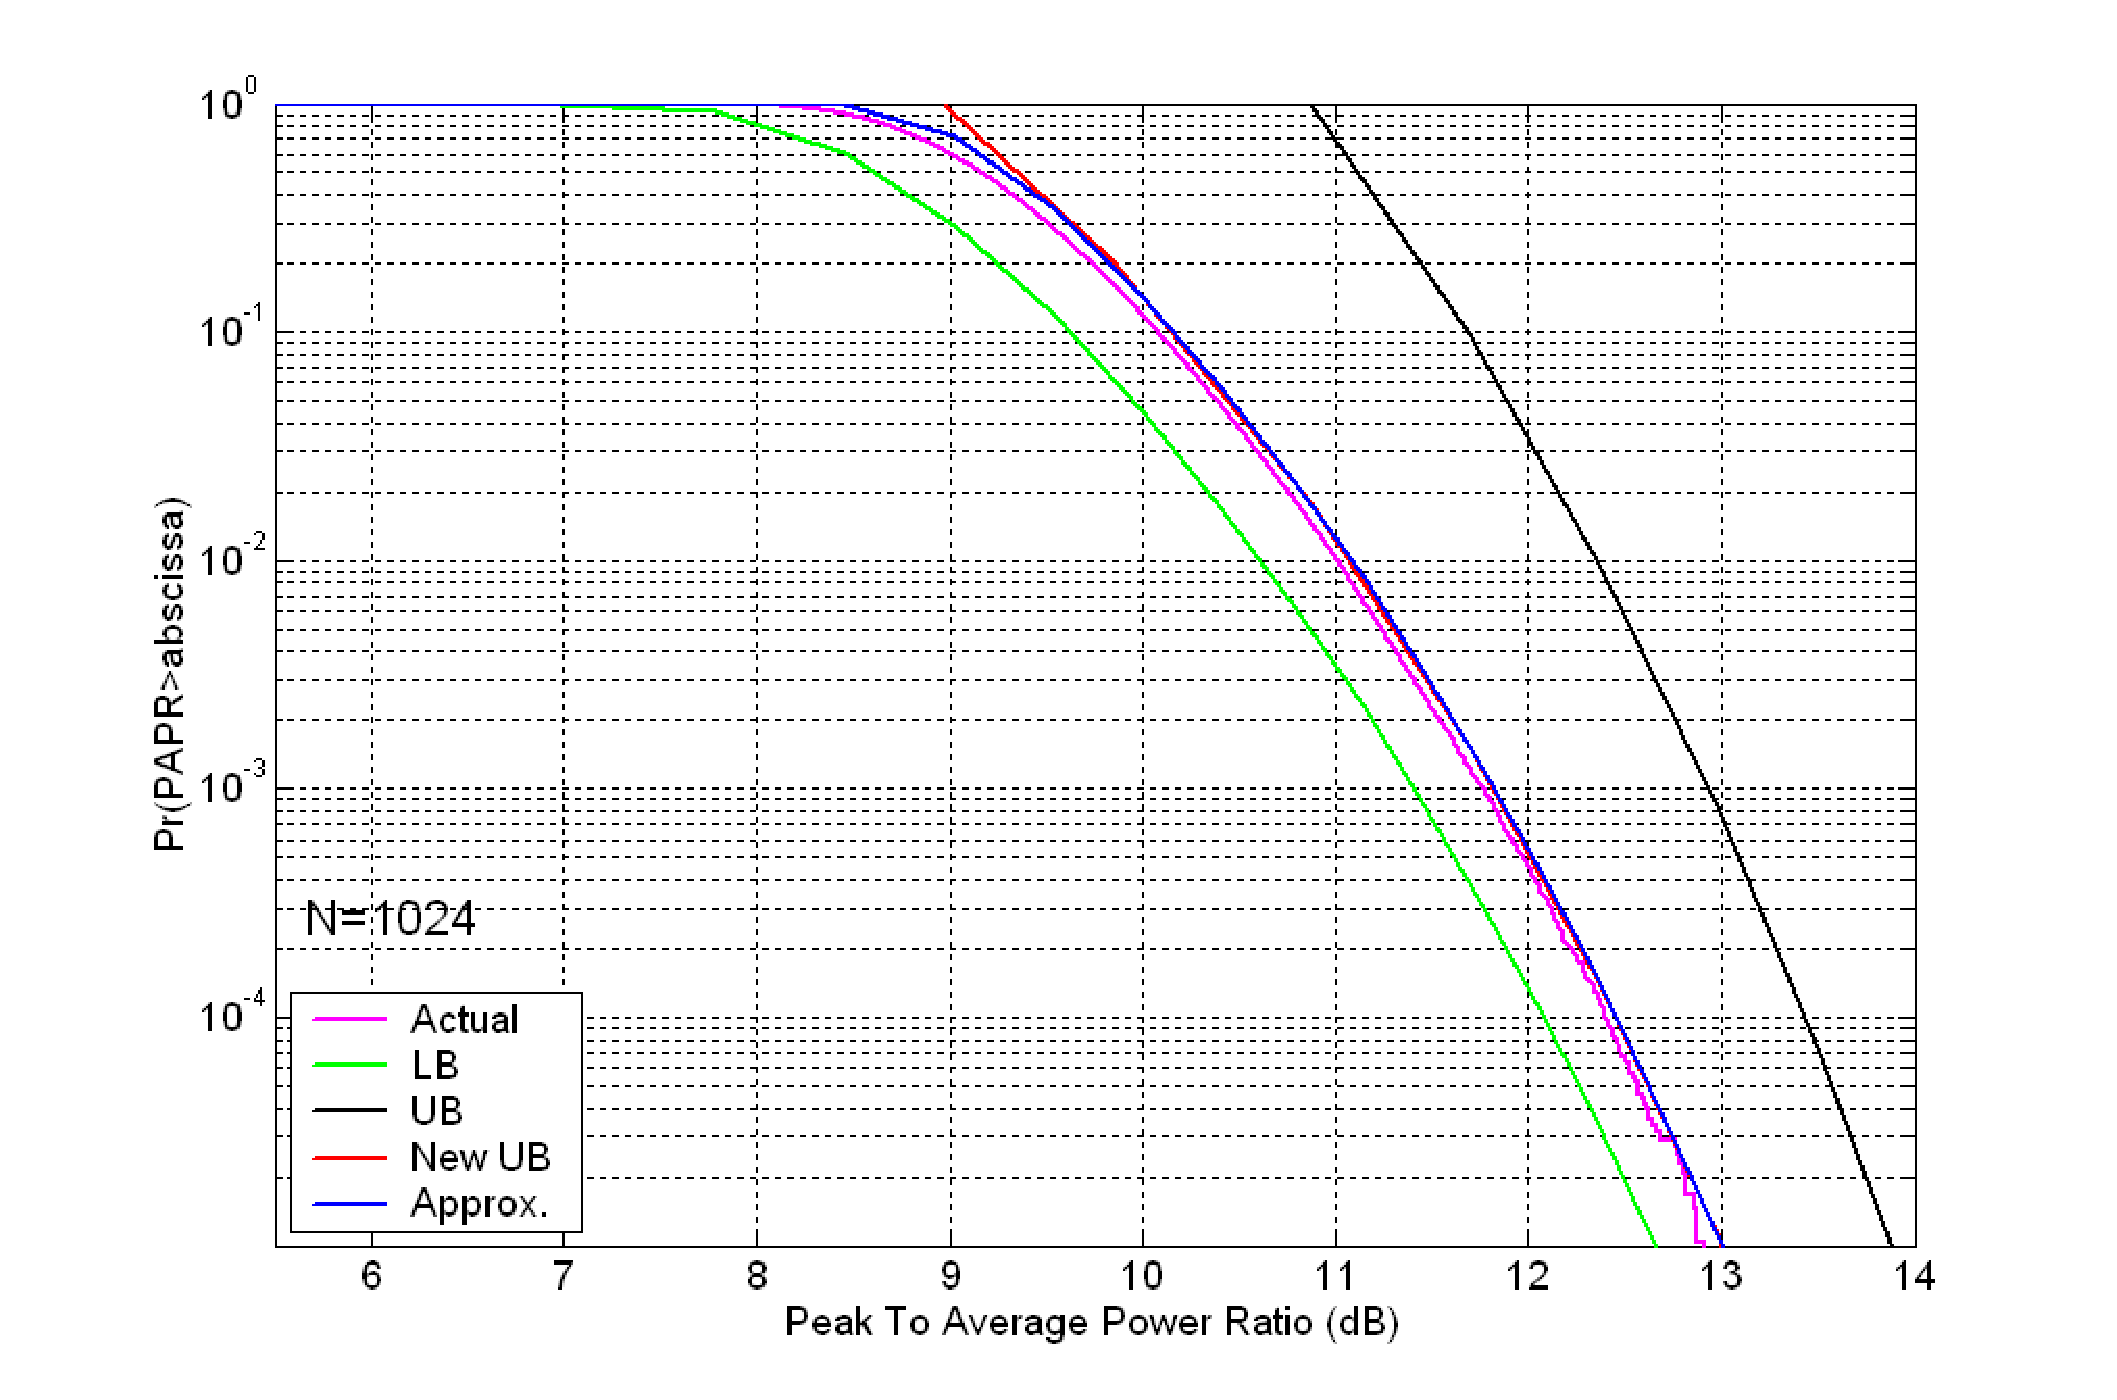
\includegraphics[width=9in,height=6in]{dist1024.pdf}} \center
Comparison of bounds and approximations (1024
subcarriers)
\begin{itemize}
\item  Simulation condition:$4$-ary QAM, $10^7 $ OFDM symbols and
oversampling rate $4$.
\end{itemize}



%slide  11 , simulation plot and condition, for 64 subcarriers
\foilhead[-0.5in]{Results-cont.} \vspace{-0.20in}
\centerline{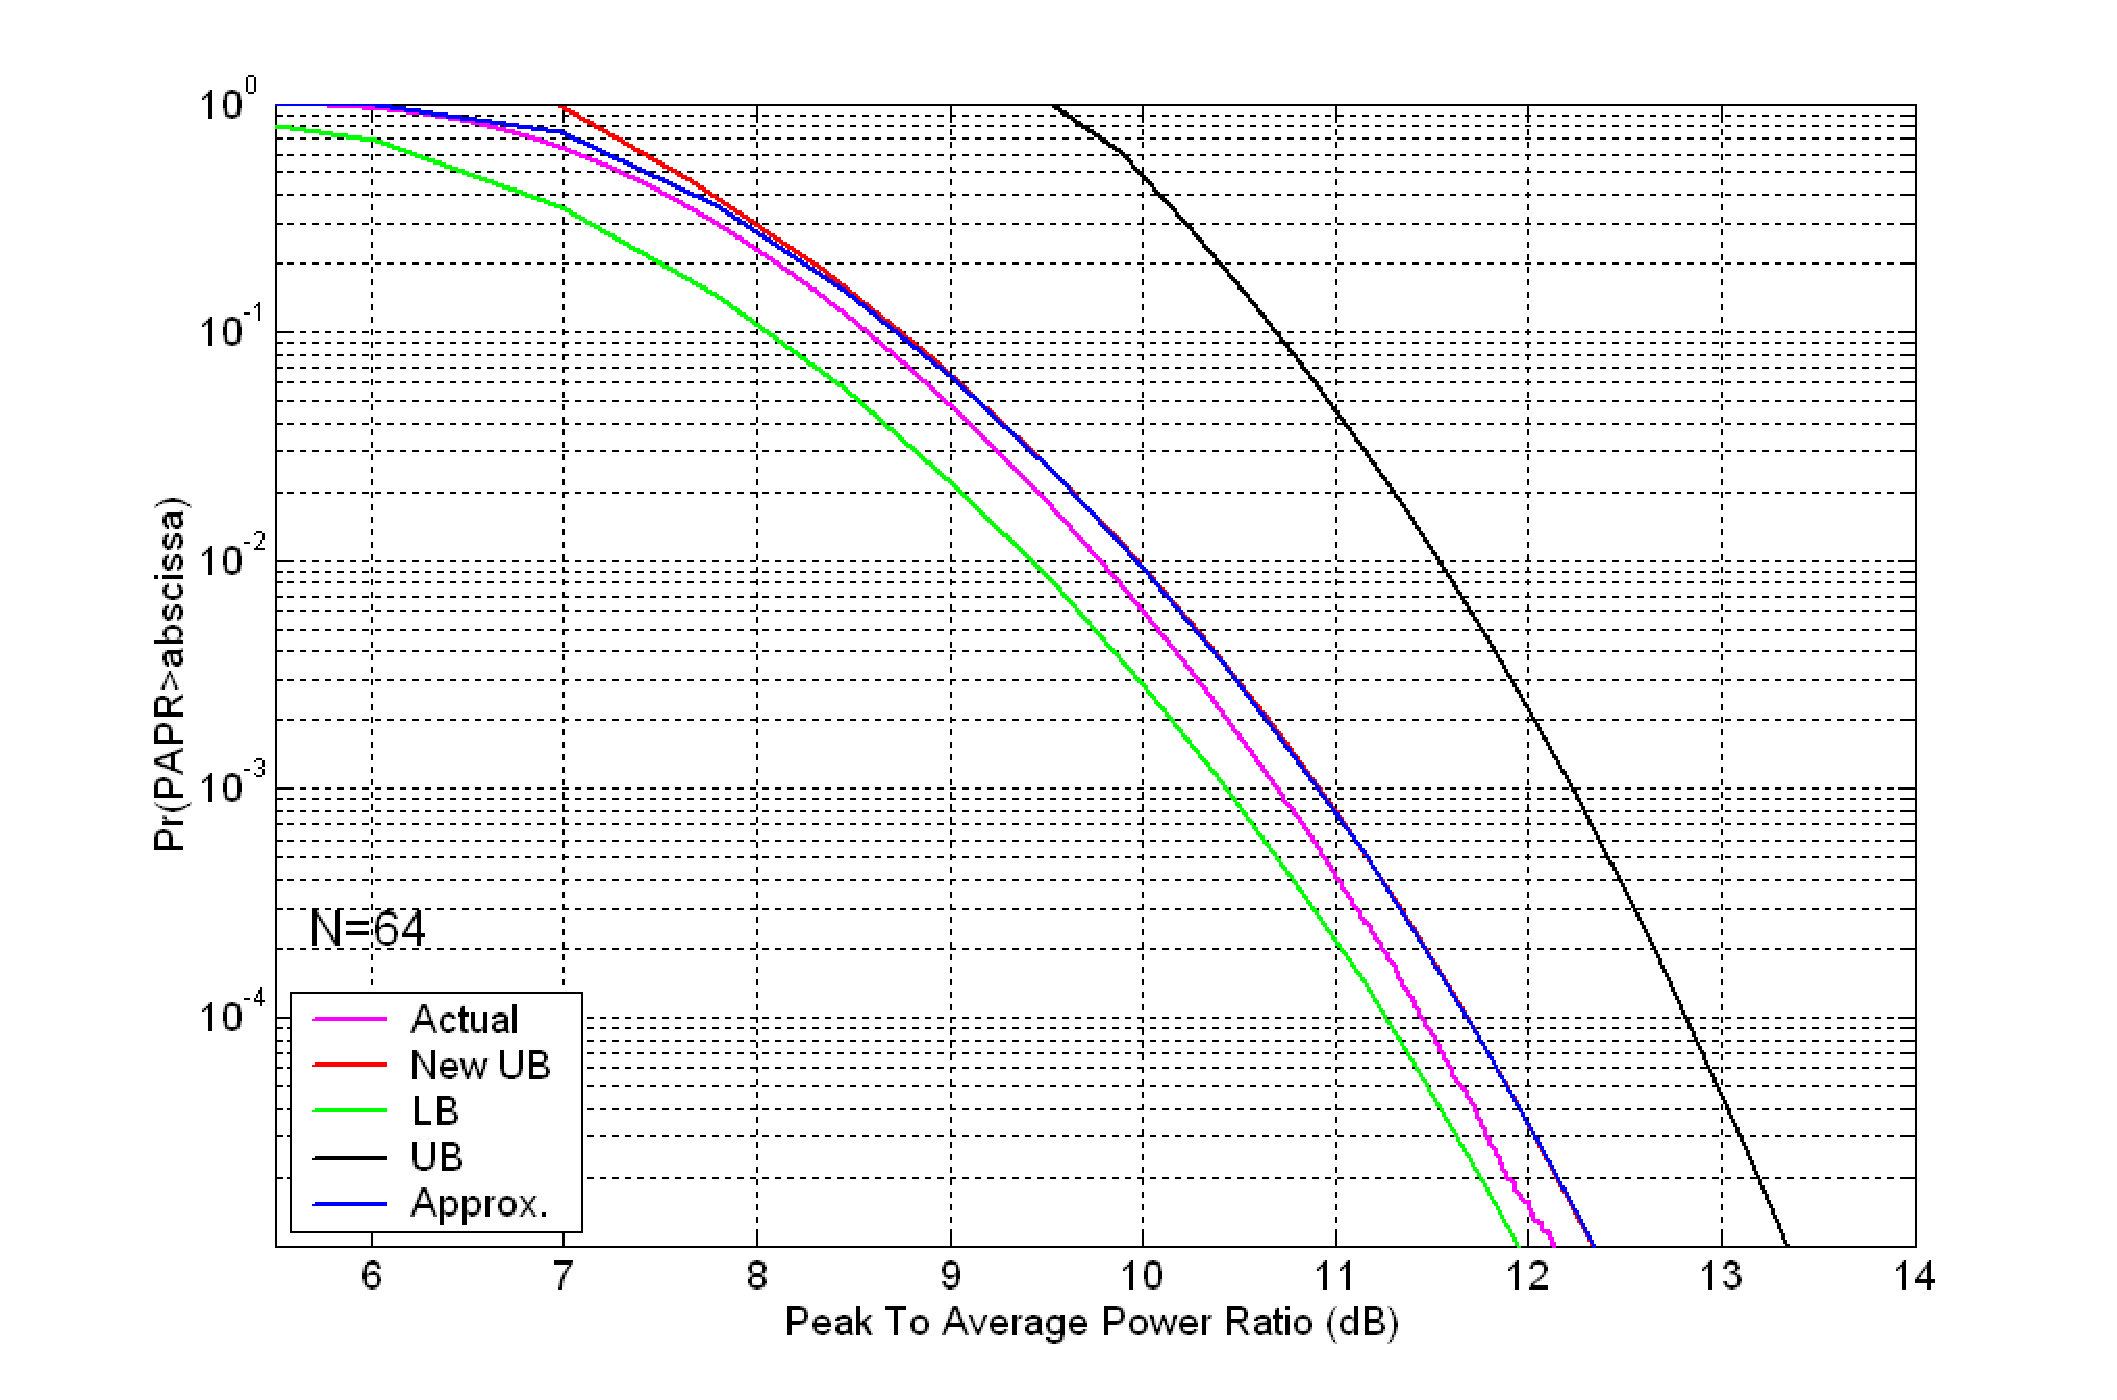
\includegraphics[width=9in,height=6in]{dist64.pdf}} \center
Comparison of bounds and approximations (64
subcarriers)
\begin{itemize}
\item  Simulation condition:$4$-ary QAM, $10^7 $ OFDM symbols and
oversampling rate $4$.
\end{itemize}



%slide 12, results, obs.

\foilhead[-0.5in]{Results Summary}
\begin{itemize}


\item The simulation shows that the proposed bound matches the
simulation results well when the subcarrier number $ \ge $ 64. The
higher the subcarrier number, the tighter the bound.

\item When the subcarrier number is 32, none of these bounds or
approximations are tight. The explanation is that $x(t)$ and
$y(t)$ are not approximated well as Gaussian random processes for
$N \le 32$.

\item The approximation in Ochiai and Imai (2001) approximates the
PAPR well if the reference $\bar \gamma$ is carefully chosen.

\item The maximum PAPR is directly proportional to the subcarrier
number $N$, however the probability of the maximum PAPR is very
small when $N\ge8$. Instead of the actual PAPR being directly
proportional to the subcarrier number $N$, we found the
$probability$ that the PAPR is greater than a given value $\gamma$
is directly proportional to the subcarrier number $N$!
\end{itemize}

% slide 13, an overview of PAPR reduction schemes
\foilhead[-0.5in]{An Overview of PAPR Reduction Schemes}
\begin{itemize}
\item Nonlinear processing \vspace{-0.20in}

\begin{itemize}
\item Clipping (or with filtering)  [Li and Cimini, 1997]

 \item
Peak windowing  [van Nee and de Wild,1998] \item Peak cancellation
[May and Rohling,1998] \item Companding [Wang and Tjhung,1999]
\end{itemize} \vspace{-0.30in}


\item Linear processing\vspace{-0.25in}
\begin{itemize}
\item Selective Mapping (SLM) [Bauml, Fischer and Huber,1996]
\item Partial Transmit Sequence (PTS) [Muller and  Huber 1997]
 \item Tone Reservation (TR) [Tellado and Cioffi 1998] \item Tone Injection (TI) [Tellado and Cioffi 1998]

\end{itemize}\vspace{-0.30in}


 \item Coding (only for small subcarrier numbers)
 [Wulich,1996]\vspace{-0.30in}


 \item Phase alignment--to choose the phase of subcarrier so that the sequence has lower
 PAPR (Newman Phase, P3 Phases and P4 Phases) [Stephen,1986][Levanon,2000].\vspace{-0.30in}

 \item
Pulse shaping function design [Slimane,2000] and dynamic
constellation (DC)[Jones,1999].\vspace{-0.30in}

\end{itemize}







%slide 14,give a brief diagram of SLM and DC seprately
\foilhead[-0.5in]{Principles of DC and SLM}

\vspace{.5in} {\small \hfill
\begin{minipage}{4.75in}
\centerline{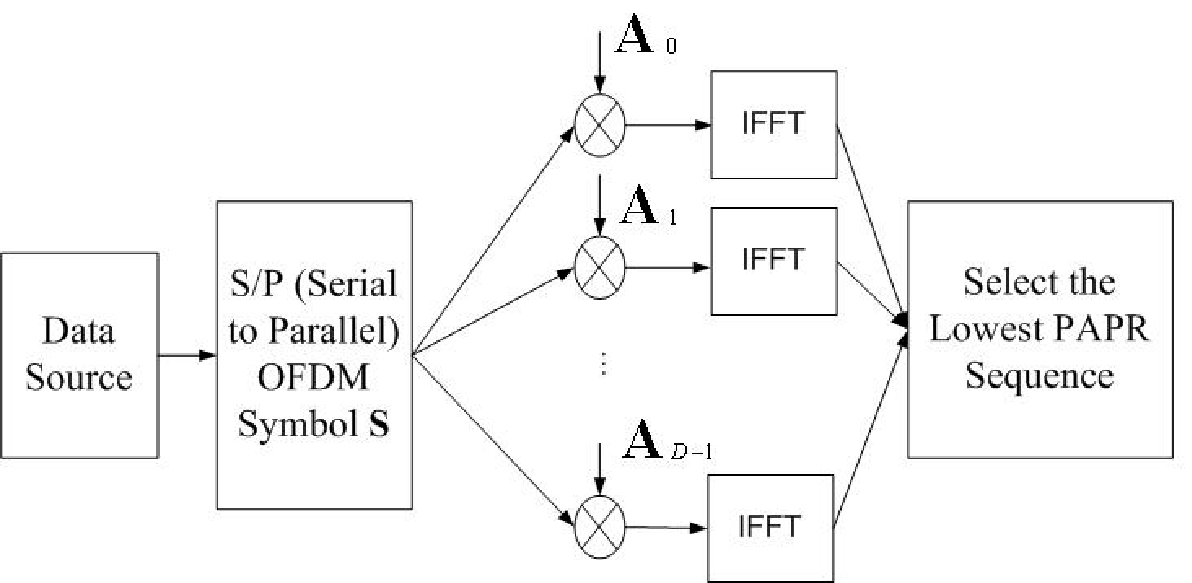
\includegraphics[width=4 in,height=3in]{slm.pdf}}
\center SLM principle.
\end{minipage}
\hfill
\begin{minipage}{4.75in}
\centerline{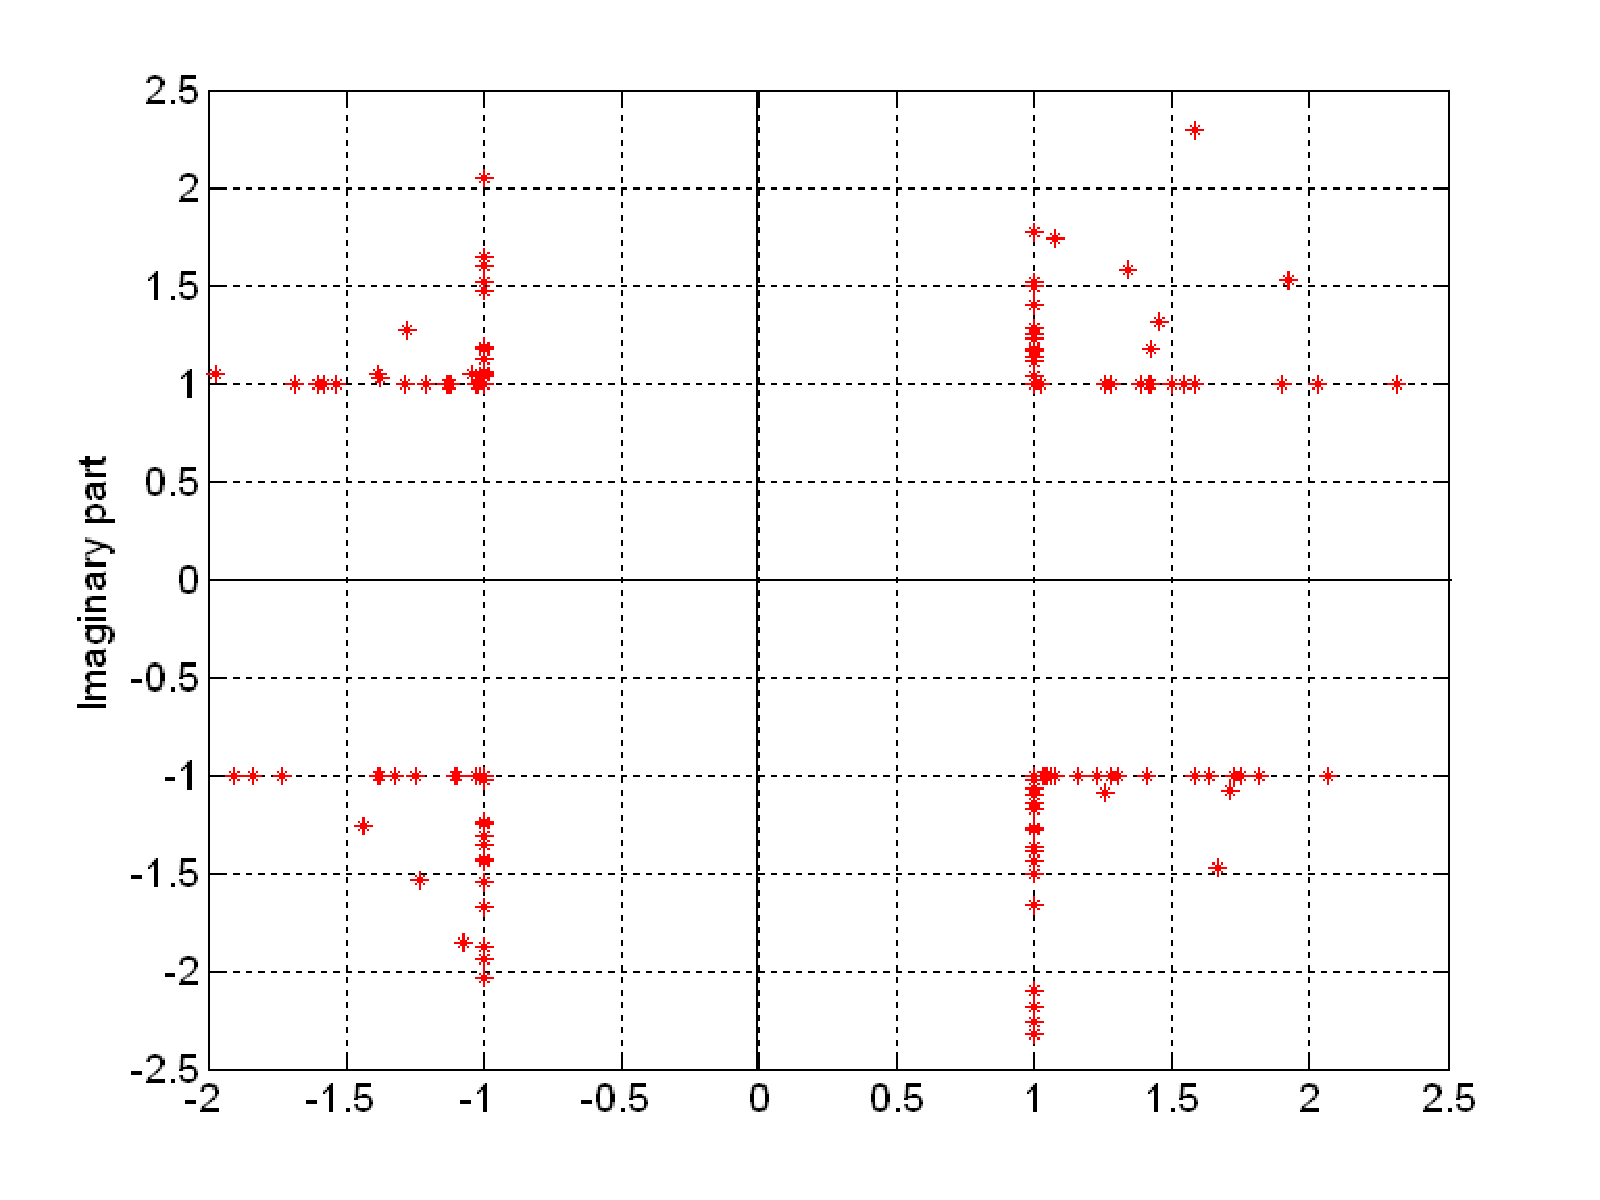
\includegraphics[width=4 in,height=3.2in]{dc.pdf}}
\center DC principle.
\end{minipage}
}

\foilhead[-0.5in]{SLM-DC for PAPR Reduction}
\begin{itemize}
\item Selective mapping (SLM) and dynamic constellation (DC) are
complementary and they benefit each other.

\item SLM: Use $D$ statistically independent sequences to
represent the same information [Bauml, Fischer and Huber, 1996].
The probability that the PAPR of SLM exceeds $\gamma$ is expressed
by $\left\{\Pr ({\rm PAPR\/}
> \gamma )\right\}^D$ where $\Pr ({\rm PAPR\/} > \gamma )$ is the PAPR
probability before using SLM and $D$ is the SLM order.

\item The dynamic constellation (DC) method
[Jones,1999] intentionally adds some noise to the input symbols so
that the PAPR is reduced. The noise is added so that each symbol
in  4-ary QAM will increase either its real or its imaginary value
so that the minimum distance between two signal points is
increased. For $4$-ary QAM modulation, we can use the projection
between the frequency domain and time domain to implement DC.
\end{itemize}



%slide 15, Limitation of SLM or DC

\foilhead[-0.5in]{Limitation of DC and SLM}
%\centerline{\includegraphics[width=3 in]{overlap.pdf}}
\begin{itemize}
\item  Limitation of DC
    \begin{itemize}
    \item Very high computational complexity\vspace{.20in}
    \item Has problem with unbalanced sequences (e.g.,
    symbols are all $1+j$).\vspace{.20in}
    \item Significant average power increase\vspace{.20in}
    \end{itemize}

\item  Limitation of SLM
    \begin{itemize}
    \item There are no ideal multiple representations for the same information in
    SLM, so we use randomly generated sequences to represent the
    same information. An order greater than $D=7$ does not provide much more
improvement for PAPR reduction.
    \end{itemize}

\end{itemize}

%slide 16, put the SLM-DC diagram here.
\foilhead[-0.7in]{SLM-DC Implementation }
\centerline{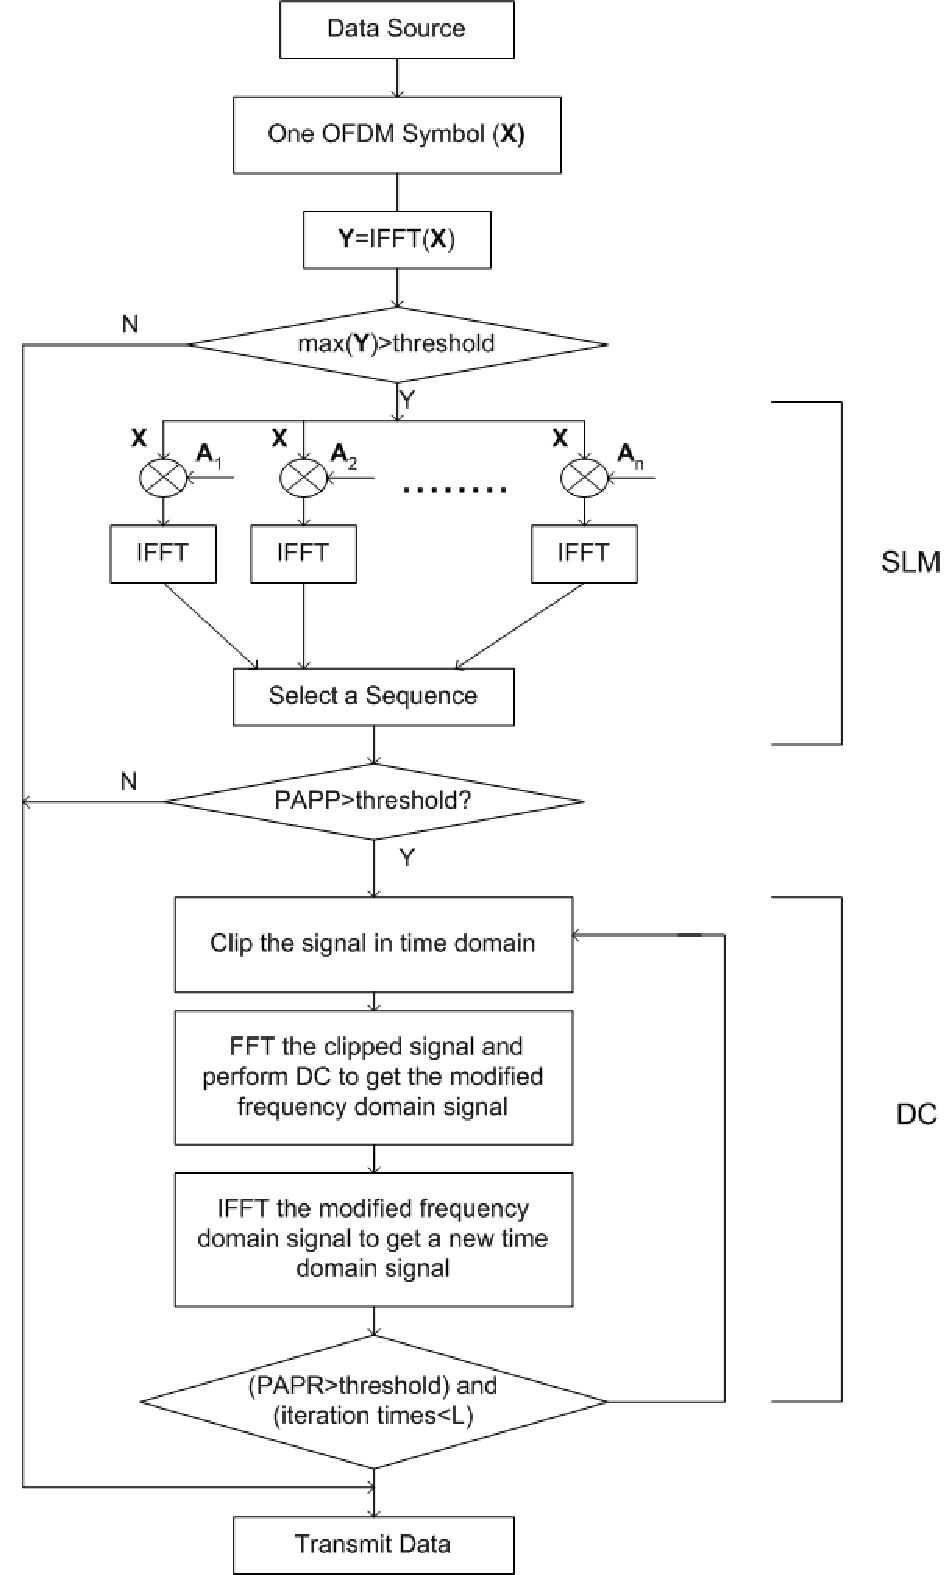
\includegraphics[width=3.5in,height=7.0in]{slmdcdia.pdf}}
%\center SLM-DC diagram



%slide 16, put the obs for SLM-DC
\foilhead[-0.5in]{Benefits achieved by combing SLM and DC}
\begin{itemize}
\item A threshold value is set to invoke SLM or DC. If a
sequence$�$s original PAPR is below this threshold, we do not use
SLM-DC and we transmit the sequence directly. Otherwise, we pass
this sequence to SLM. If after using SLM, the PAPR is below the
threshold, we transmit the sequence directly without DC.
Otherwise, we further employ DC to reduce the PAPR. This method
has less overall computational complexity compared to DC only.

\item Reduce average-power-increase; without SLM, DC only will
increase the  average power significantly!If we take the threshold
to be 7.7 dB for 128 subcarriers, the average power increase will
be about $0.25\%$ for 7$^{th}$ order SLM-DC. In the case without
SLM, DC will have an average power increase of  $40\%$.

\item SLM makes the input sequence more randomly located in the
signal space so that DC's ability to reduce PAPR is extended.

\item More PAPR reduction.

\end{itemize}



%slide 17, an example shows the SLM extends DC ability
\foilhead[-0.5in]{SLM extends DC's ability }\vspace{0.4in}
\centerline{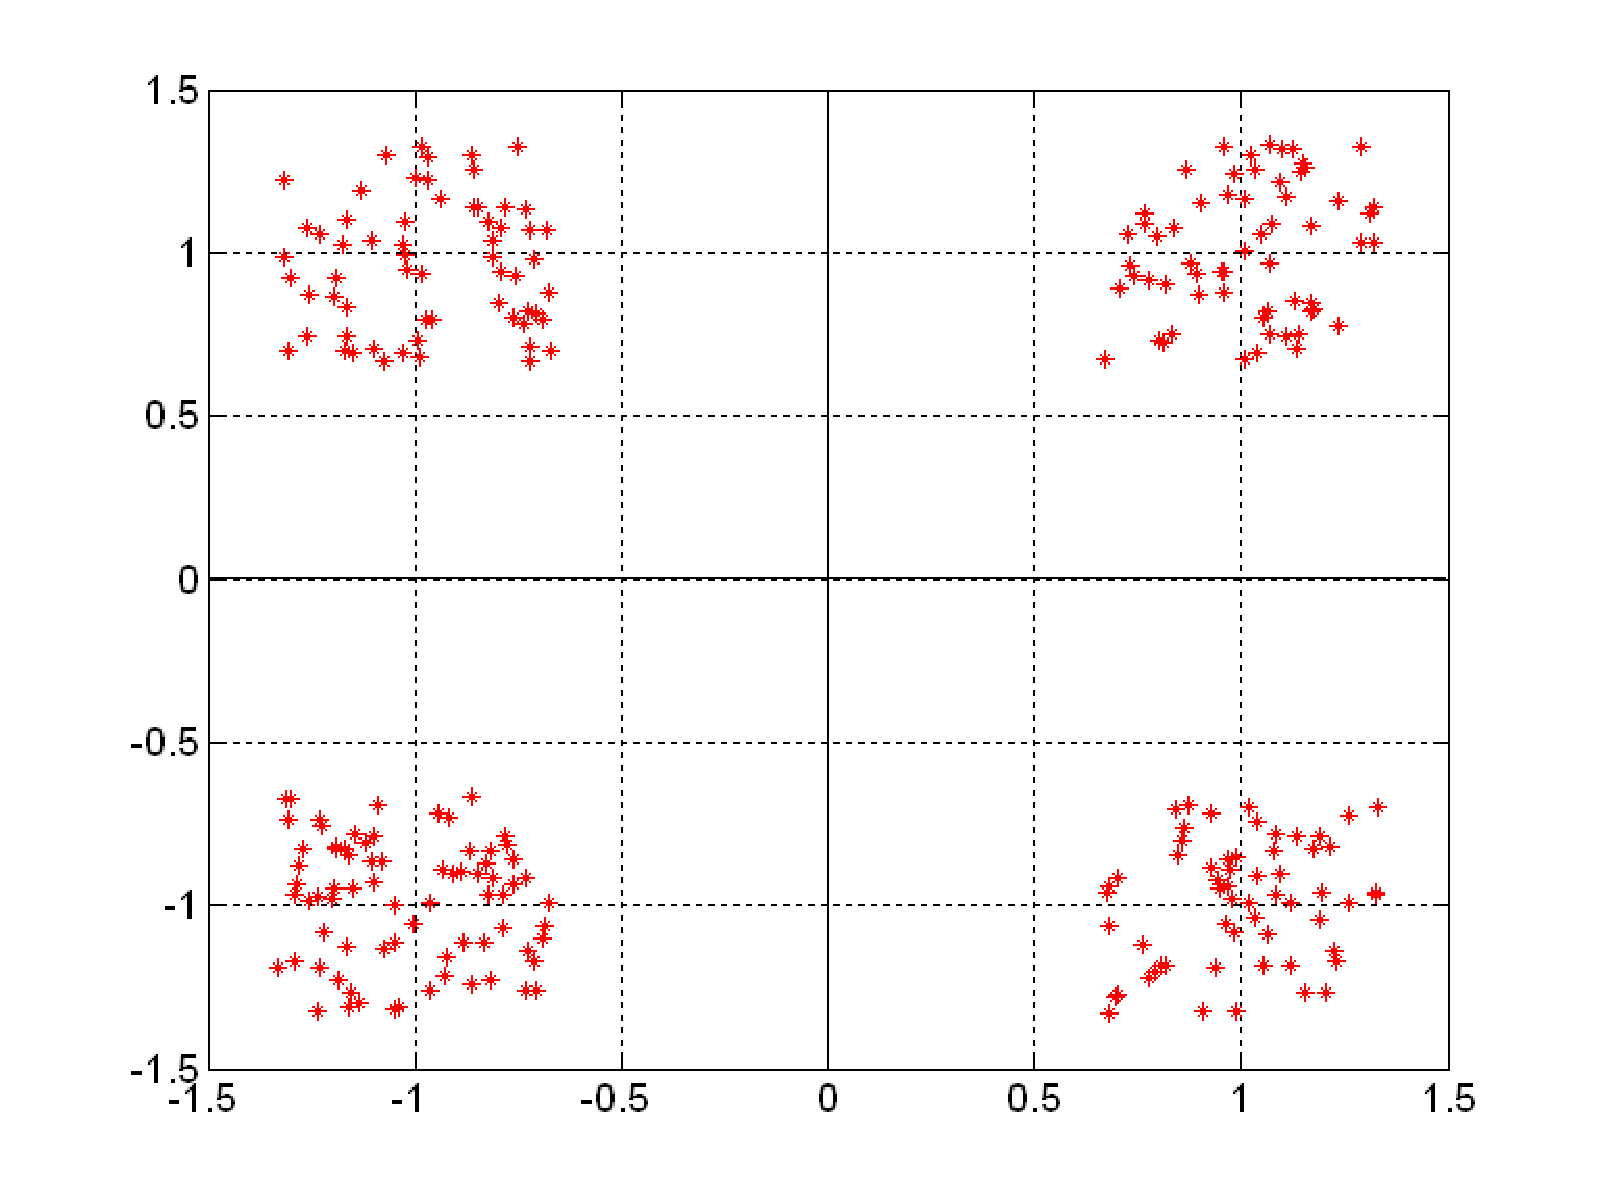
\includegraphics[width=5 in]{balance.pdf}} \center SLM
extends DC's ability by making symbols balanced.
\begin{itemize}
 \item  SLM-DC can work on all $1+j$ sequences. The sequence has balanced symbols (as shown in the plot) after SLM and the PAPR is reduced
 from 24 dB to 8 dB ($N=256$), further the DC works on the balanced sequence and the final
PAPR will be as low as 4.8 db ( Threshold value is 4.77. dB and 7th order SLM-DC).
\end{itemize}


%slide 18 Effect of SLM-DC for PAPR reduction
\foilhead[-0.5in]{Effects of DC combined with SLM}\vspace{0.4in}
\centerline{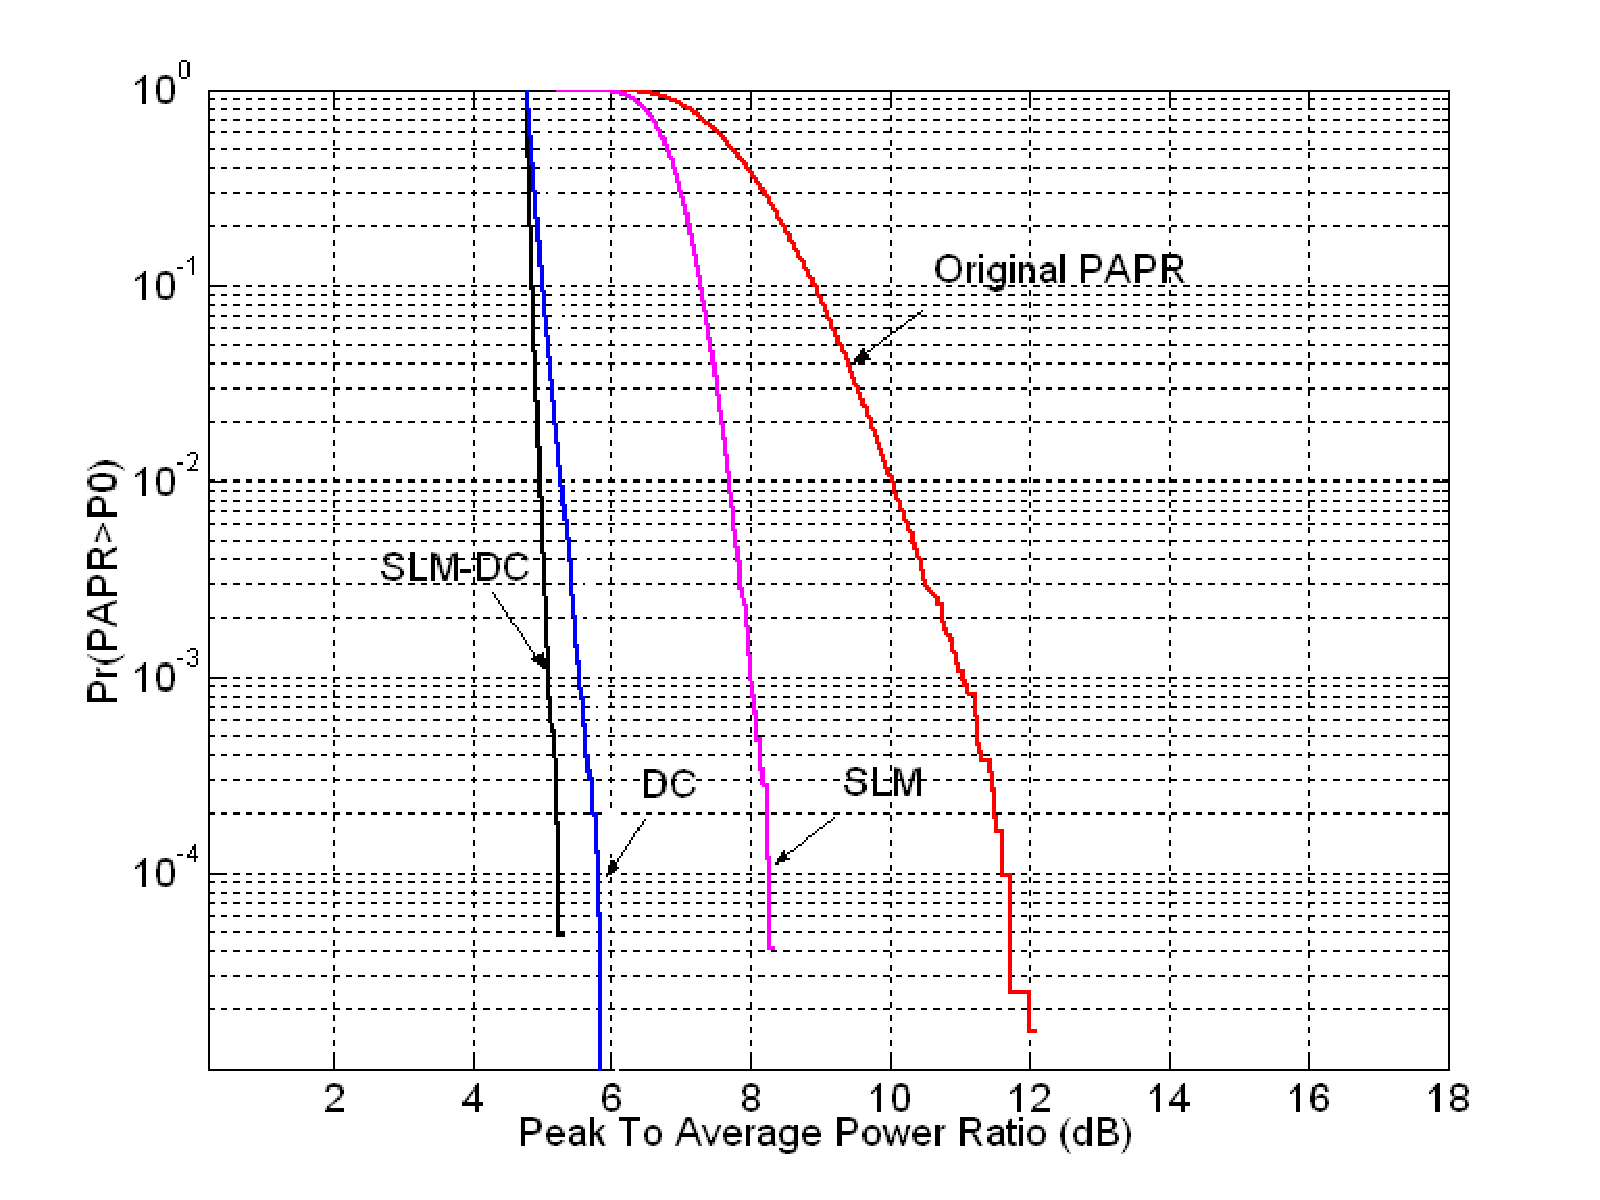
\includegraphics[width=5in]{slmdc.pdf}} \center Effect
of DC combined with SLM.
\begin{itemize}
 \item In this example of a 128-subcarrier OFDM system, it reduces the PAPR at a probability
of $10^{ - 4}$ from 11.8 dB to 5.2 dB. The reduction is 2 dB more
than SLM and 0.5 dB more than DC.\vspace{-0.25in} \item SLM-DC
slightly better than DC but with much less overall computational
complexity, less average power increase and extended ability for
unbalanced sequences.
\end{itemize}



%slide 19 conclusion.
\foilhead[-0.5in]{Conclusions}
\begin{itemize}
\item A new simpe bound on the PAPR distribution in OFDM  is
proposed in this paper and our simulations show that this bound is
tight when the subcarrier number $N$ is greater than 64.

\item The $probability$ that the PAPR is greater than a given
value is directly proportional to the subcarrier number $N$.

\item We proposed SLM-DC for PAPR reduction and simulations show
that this combination achieves good PAPR reduction.

\item An estimate of the average power increase in SLM-DC via the
proposed bound shows that SLM-DC can reduce the average power
increase significantly, compared to DC only.


\end{itemize}



\end{document}
